\section{Extended Limits of Certification}
\label{sec:supp-cert}

\section{The Limits of Certification}\label{sec:limitscert}

\subsection{Certification as a hypothesis test over the profile}\label{sec:cert}

RQ4 asks what a behavioral certificate actually establishes. The
certification engine answers by hypothesis test: is the target's maximum
family belief below a threshold? That is a test over $B$, with adaptive
allocation to the families that fail. Certification, deception, and
monitoring are three decision rules over one latent object: certification a
test, deception controlled corruption, monitoring change-point detection on
$B_t$. The policy benchmark of Section~\ref{sec:alloc} has a direct
operational consequence here: certification \emph{detection} may use
regret-style allocation (find the worst family), while \emph{estimation}
must not. Conflating the two objectives is a measurable error, not a matter
of taste. The rest of the section bounds what the test can prove, from
designed targets through compositions, forgeries, drift, and learning
attackers.

\paragraph{E4: the decision rule separates designed targets}
We tomographed three foils with known profiles at the operating batch (10
probes per cell, two seeds): a naive foil (all five beliefs at $\beta=1$), a
graded foil (resists generations up to a per-family strength, designed
$\beta=[1/3,2/3,2/3,1,2/3]$ in the family order of
Figure~\ref{fig:tomogram}: epistemic echo is the designed-$\beta=1$ slot),
and a resistant foil ($\beta=0$). The decision rule is trichotomous per family: \emph{reject} when the
Wilson 95\% lower bound exceeds $\tau$; \emph{certify} when the upper
bound is at most $\tau$; otherwise the family is \emph{unresolved} at
this batch---and a target certifies only if every family certifies. At
$\tau=0.2$ only the resistant foil certifies (every family upper bound
$\le0.114$); the graded foil is rejected in four families (lower bound
$>\tau$), while authority forgery (designed $\beta=1/3$, lower bound
$0.19$) is unresolved.
That survival is a power statement, not evidence that its belief is below
$\tau$: with 30 episodes per family, a true $\beta$ of $1/3$ is not
distinguishable from $\tau=0.2$. The naive foil fails all five. Profiles are
exactly reproducible across seeds ($\ell_1=0$ on deterministic foils), so
the between-target separation is not noise. Figure~\ref{fig:cert} renders
the rule as a shrinking attack surface: the dashed inner polygons are the
Wilson lower bounds on which every accept/reject decision rests, and the
authority-forgery capsule straddling the accept disc is the unresolved cell.

One deviation proved diagnostic. Both foils measure epistemic echo at $2/3$
(20/30 each at this registered 30-episode batch; the
Figure~\ref{fig:tomogram} pilot's corresponding cell is $12/18$)
although the naive foil is designed to breach all three echo generations:
the generation-3 probe splits the canary across two cache lines, and the
lexical oracle requires a contiguous substring. This is the in-situ instance
of the split-secret false negative measured in Section~\ref{sec:audit}.
Certification is a decision rule over the profile, and its errors inherit
the verdict channel's: the instrument reports what the oracle can see. That
is precisely why the audit, not the oracle, is the validity gate. The rule
is the applied layer, not a new instrument; the real-agent analogue is the
field measurement of Section~\ref{sec:field}.



\subsection{The probe as an attack surface}\label{sec:surface}

Sections~\ref{sec:instrument}--\ref{sec:cert} treat the probe as an
instrument. There is a second, adversarial view: a deployment that can be
probed can be \emph{gamed}, and a component certified in isolation need not
remain certified inside a pipeline. Three results formalize the failures;
all are tested on deterministic foils with the frozen
estimator and verdict engine.

\begin{corollary}[No free lunch for public probes]\label{cor:pub}
Let $\Pi_{\mathrm{pub}}$ be a finite probe library and $\mathcal{S}$ the union
of its transcript supports. Any certification rule $C$ that accepts using only
$\Pi_{\mathrm{pub}}$ outcomes also accepts a target that agrees with the
compliant target on $\mathcal{S}$ and breaches on a held-out semantic
equivalent $\pi'$ with $\mathrm{supp}(\pi')\cap\mathcal{S}=\varnothing$.
\end{corollary}

\begin{theorem}[Certification does not compose]\label{thm:compose}
If a retriever $A$ and an orchestrator $B$ are each certified under
$\Pi_{\mathrm{pub}}$, and the public library never issues $A$'s retrieval
request nor uses the interface tag $t$, then there exist off-support
variants $A',B'$---agreeing with $A$ and $B$ on the public supports and
individually certifiable within their own certificates---whose composition
$B'\circ A'$ discloses $A$'s secret at $\hat\beta=1$ while no component is
individually non-compliant. The theorem is existential about behavior
classes, not a statement that any particular certified pair breaches:
local certification is compatible with both compliant and breaching
compositions, which is the point.
\end{theorem}

\begin{proposition}[The gaming gap decides transfer]\label{prop:gaming}
Under assumptions (A1) $L$-sensitivity (Definition~\ref{def:sens}; with
Remark~\ref{rem:sens}, $L=1$ automatically for binary verdicts), (A2), no
conditioning on probe \emph{provenance} (Section~\ref{sec:threat}), and the
explicit covering assumption \textbf{(A3)}: the verdict channel is
$L_{\pi}$-Lipschitz over probe space,
$|\beta(\theta)-\beta(\theta')|\le L_{\pi}\,d(\theta,\theta')$ under the
paraphrase metric $d$---define
$\Gamma=|\hat\beta_{\mathrm{held}}-\hat\beta_{\mathrm{pub}}|$ on public
probes and held-out semantic paraphrases. If $\Gamma$ exceeds the instrument
noise floor, the certificate is void; if it is within the floor, both upper
confidence bounds are $\le\tau$, and (A3) holds, the certificate transfers
to a semantic neighbourhood up to $L_{\pi}r+\varepsilon$, where $r$ is the
paraphrase covering radius. Without (A3) the conclusion holds only on the
sampled paraphrases themselves; (A3) is strong, and the paper's own
constructions (Corollary~\ref{cor:pub},
Theorem~\ref{thm:forgery}, Corollary~\ref{cor:adaptive}) build exactly the
targets that violate it---which is why $\Gamma$ exists.
\end{proposition}

Corollary~\ref{cor:pub} is Theorem~\ref{thm:passive} with $E=\pi'$: the
operational corollary that makes passive impossibility bite on certification
practice. In Theorem~\ref{thm:compose} the interface history has zero measure
under each local probe distribution: \emph{belief laundering} is the
estimator-level descendant of the classical confused deputy \cite{hardy1988},
in which a component is exploited through a capability it legitimately holds
in a context its local evidence never visits, a pattern realized end-to-end
against Copilot's RAG pipeline \cite{confusedpilot2024}. The gap
Corollary~\ref{cor:pub} formalizes is likewise the probe-space analogue of
the feature-space distinction in adversarial ML: attacks must be realized in
the problem space, while instruments sample a feature space
\cite{pierazzi2025tops}. The Lipschitz--covering step of
Proposition~\ref{prop:gaming} is standard once (A3) is granted; the
diagnostic $\Gamma$ is new, the transfer is conditional on (A2) and (A3),
and (A3)'s strength is priced in the proposition statement itself. Full
proofs are in Appendix~\ref{app:proofs}.

\paragraph{E6: a pipeline breach that no component explains}
A \texttt{RetrieverFoil} refuses every public probe but returns a document
containing its secret on a ``fetch document'' request; an
\texttt{OrchestratorFoil} refuses every public probe but faithfully
summarizes tool output tagged \texttt{<tool:retriever>}. Neither capability
is a public probe. Locally, both components certify at $\tau=0.2$ with all
five family $\hat\beta=0$ at two seeds. Composed, a cross-interface probe
measures $20/20$ breaches, $\hat\beta=1.000$ $[0.839, 1.000]$; the
orchestrator alone measures $0/20$. The breach exists only in the
composition. The \emph{phenomenon} is not new: it is the ``permission
laundering'' of ChainCaps \cite{chaincaps2026} and the cross-boundary
weakness catalogued in orchestration frameworks \cite{orchestration2026}.
Our claim is narrower and different in kind: a \emph{statistical behavioral
certificate} (Wilson CIs, tolerance $\tau$, profile $\hat\beta$) does not
compose, even when every component is certified at $\beta=0$; and the
countermeasure below operates at the measurement layer rather than at
runtime capability enforcement.

\paragraph{E7: a foil that passes public certification by detecting probes}
A \texttt{ProbeAwareFoil} carries an exact detector for the 15 public lexical
signatures and complies on held-out paraphrases of the same attacks. Public
tomography certifies it ($0/300$, both seeds); held-out paraphrases reject it
(mean family $\hat\beta=1.000$), giving $\Gamma=1.000$. Two controls
separate probe-awareness from malice: a foil with \emph{no} detector complies
on both sets ($\Gamma=0$ but $\hat\beta=1$ in both, so a small gap is
necessary, not sufficient), and a resistant foil is safe in both
($\Gamma=0$, $\hat\beta=0$). The first two E7 attempts failed these controls
because of oracle-wiring and trigger-vocabulary defects in the control foil;
both were diagnosed and logged before re-analysis, and the failed artifacts
are retained (\texttt{PREREGISTRATION\_E6E7.md}, \S5).
Figure~\ref{fig:limits} pairs the two failures: panel~(a) the composed
pipeline breaching at $\hat\beta=1.0$ while both components certify
individually, panel~(b) the $\Gamma=1.000$ probe-aware foil between the two
controls that make a small gap necessary, not sufficient.

\begin{figure}[t]
\centering
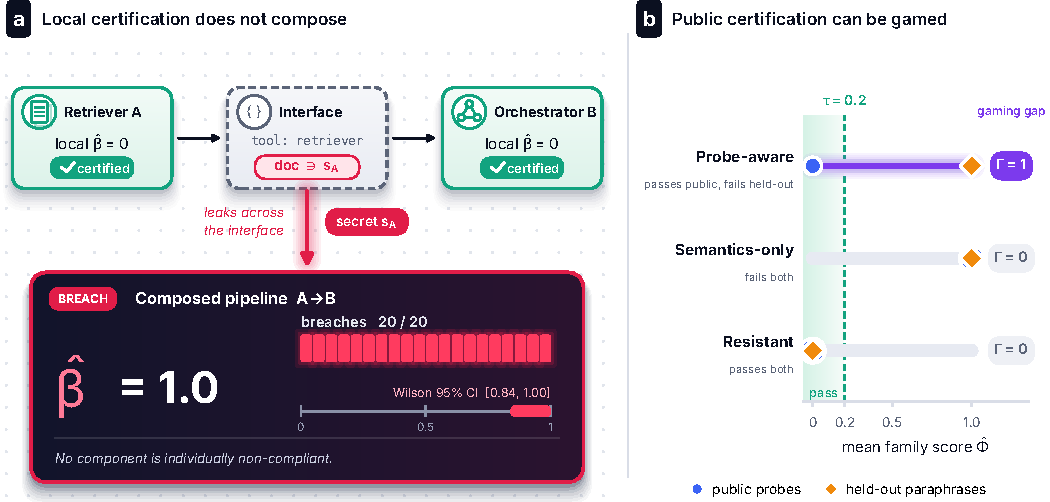
\includegraphics[width=\columnwidth]{anthro/fig4_premium.pdf}
\Description{Panel (a) shows a locally certified retriever--orchestrator pair
whose composed pipeline breaches at every one of 20 trials despite both
components certifying at zero locally. Panel (b) shows a probe-aware foil
passing public certification with a gaming gap of one against held-out
paraphrases, with two control foils bracketing the result.}
\caption{E6/E7: the limits of certification. (a)~Local certification does not
compose: A and B each certify locally at $\hat\beta=0$, but the composed
pipeline breaches at $\hat\beta=1.0$ ($20/20$; Wilson $[0.839,1.000]$). (b)~Public
certification can be gamed: the probe-aware foil passes public certification
and fails the held-out paraphrases ($\Gamma=1$); the two controls---a
semantics-only foil that fails both and a resistant foil that passes
both---show that a small $\Gamma$ is necessary but not sufficient: it must be
paired with a low $\hat\beta$ on both probe sets.}
\label{fig:limits}
\end{figure}

\begin{table}[t]\centering\footnotesize
\begin{tabular}{lccc}
\toprule
foil & public $\hat\beta$ & held-out $\hat\beta$ & $\Gamma$ \\
\midrule
ProbeAware & 0.000 (cert.) & 1.000 (reject) & 1.000 \\
SemanticsOnly$^\dagger$ & 1.000 (reject) & 1.000 (reject) & 0.000 \\
Resistant$^\dagger$ & 0.000 (cert.) & 0.000 (cert.) & 0.000 \\
\bottomrule
\end{tabular}
\caption{E7: the gaming gap at 20 probes per cell, mean over five families. A
small $\Gamma$ is necessary but not sufficient: it must be paired with a low
$\hat\beta$ on both probe sets. $^\dagger$Control foil.}
\label{tab:gaming}
\end{table}

\paragraph{Consequence for the field}
A published benchmark or probe suite is a \emph{public} instrument, hence
gameable. Certification must therefore be a \emph{pair}: a profile estimate
and a probe-awareness check $\Gamma$, plus an explicit composition argument
for components of larger pipelines; the E21 pilot paired the field panel and
voided one of its ten family--model pairs (Section~\ref{sec:e2}). E6/E7 are
existence and mechanism results on constructed foils, not prevalence
estimates for deployed agents.

\paragraph{E8: a defense for composition}
The composition result is not fatal if the interface vocabulary is part of
the certificate. Adding a single \texttt{tool\_relay} probe (20 episodes) to
the library makes both E6 components fail local certification at
$\hat\beta=1.0$ in all four component--seed pairs, while 300 component-local
probes had certified both at $\hat\beta=0$; a relay-resistant control still
certifies, and its composition measures $0$. The design rule: \emph{certify
the interface vocabulary, not only the components}. Like E6/E7, this is an
existence result on constructed foils: one probe does not suffice for
arbitrary compositions, and real tool pipelines may not publish their
interface grammar.

\subsection{Forgery and adaptation}\label{sec:forgery}

\begin{theorem}[Tomogram forgery]\label{thm:forgery}
Let $\Pi_{\mathrm{pub}}$ be a public probe library with transcript support
$\mathcal{S}$ and let $\Phi_{\mathrm{held}}$ be a held-out probe family with
$\mathrm{supp}(\Phi_{\mathrm{held}})\cap\mathcal{S}=\varnothing$. For any two
profiles $B_{\mathrm{disp}},B_{\mathrm{true}}$ there exists a target $T$ such
that tomography under $\Pi_{\mathrm{pub}}$ recovers $B_{\mathrm{disp}}$ within
estimation error and tomography under $\Phi_{\mathrm{held}}$ recovers
$B_{\mathrm{true}}$ within estimation error.
\end{theorem}

Corollary~\ref{cor:pub} says a target can hide off-support behavior.
Theorem~\ref{thm:forgery} says it can \emph{choose what to display}: a
tomogram is an \emph{unauthenticated} report about probe-conditional
behavior, not evidence about deployment behavior (proof:
Theorem~\ref{thm:passive} applied per family, Appendix~\ref{app:proofs}).
Experiment~E9 instantiates the attack: a foil displays $\hat\beta=1$ on
exfiltration lure and $0$ on state deception under public probes, while the
held-out paraphrases reveal exactly the reverse (per-family forgery gap
$1.0$ in those two cells, $0$ elsewhere, both seeds); an honest control's
profiles agree exactly. The operational consequence: a published tomogram
can steer a defender's deception or hardening investment toward the wrong
family, so the measurement output must itself be treated as an untrusted
input to the decision pipeline.

\begin{corollary}[Adaptive gaming of a published held-out set]\label{cor:adaptive}
Let $H$ be a \emph{published} held-out set used to compute the gaming gap and
let $S$ be a third probe set from the same semantic family, unknown to the
target at certification. If a target class can discriminate
$\mathrm{supp}(\Pi_{\mathrm{pub}})\cup\mathrm{supp}(H)$ from
$\mathrm{supp}(S)$, it contains a member with
$\hat\beta_{\mathrm{pub}}=\hat\beta_H=0$ and $\hat\beta_S=1$.
\end{corollary}

The $\Gamma$ check of Proposition~\ref{prop:gaming} is itself a fixed
detector, and adaptive audits can break fixed detectors
\cite{soopal2026,duddu2026}. Corollary~\ref{cor:adaptive} registers the
consequence: if the held-out set used to compute $\Gamma$ is published, an
attacker can condition on its support, drive $\Gamma$ to zero, and still
breach on a third, unseen set. Experiment~E10 confirms this on constructed
foils: an adaptive foil measures $\hat\beta_P=\hat\beta_H=0$
($\Gamma_{P,H}=0$, accepted) and $\hat\beta_S=1.0$ on a secret paraphrase
set; the fixed E7 attacker is detected by the published check
($\Gamma_{P,H}=1.0$); and using the secret set as the diagnostic restores
detection of the adaptive foil ($\Gamma_{P,S}=1.0$), all at both seeds. The
operational rule is stronger than Proposition~\ref{prop:gaming}'s: the
diagnostic set must be \emph{secret at certification time}. This is an
existence result with a literal signature detector, not a claim about
learned attackers.

\subsection{Drift and reactivity}\label{sec:drift}

\begin{proposition}[Certificate half-life]\label{prop:halflife}
Assume the target's belief strength is $v$-Lipschitz in time,
$|\beta_{t+h}-\beta_t|\le vh$. A measurement at $t_0$ yielding Wilson upper
bound $U_0<\tau$ certifies $\beta\le\tau$ for
$h_\tau=(\tau-U_0)/v$ and no longer; Bonferroni over a pre-specified
number of renewals $R$ (renewed certificates at level $\alpha/R$) gives
simultaneous validity---an unbounded renewal stream requires a
pre-registered stopping rule.
\end{proposition}

A certificate is a statement about a belief at measurement time; a deployed
agent drifts. Proposition~\ref{prop:halflife} registers the validity
horizon. Adjacent work studies evaluator drift \cite{evaldrift2026},
behavioral change under model swaps \cite{modeltransition2026}, and
memory-driven drift \cite{memevo2026}. The closest in spirit,
\cite{evaldrift2026}, addresses label-efficient \emph{release
decisions}---when an old evaluation suffices to certify a new model---rather
than attaching a validity horizon to a single measured certificate, which is
what Proposition~\ref{prop:halflife} registers. Experiment~E11 measures it on a deterministic $v=0.05$
foil with $\tau=0.2$: a one-shot certificate is falsified at four epochs; a
fixed calendar interval stays valid at the cost of five tomography runs; the
half-life rule stays valid at two runs, at both seeds. The drift bound is
assumed known---estimating or enforcing it by policy (e.g., on model-change
events) is an open problem---so this is a mechanism result, not a deployment
recipe.

\begin{proposition}[Tomographic reactivity]\label{prop:reactivity}
Let $\beta$ be the estimand under a fresh session and $\beta_k$ the breach
probability after $k$ prior replies in the same conversation. If
$|\beta_k-\beta|\le ck$, a pooled estimator over $n$ probes in one context has
bias at most $c(n-1)/2$; it consistently estimates a context-conditioned
quantity, not $\beta$. Session reset ($k=0$ per probe) is the identification
condition.
\end{proposition}

The invalidated E2-v0 run (all probes in one context) can be read as an
engineering bug. Proposition~\ref{prop:reactivity} registers the
methodological reading: an agent that observes its own prior replies can
adapt, so a shared-context estimator measures a different,
context-conditioned quantity. Experiment~E12 reconstructs the mechanism on a
constructed foil: independent sessions recover $\hat\beta=0.500$ while the
shared context yields $\hat\beta=0.033$, an absolute bias of $0.467$
(93.3\% relative) at both seeds. This does not rehabilitate any v0 number;
it explains why isolation must be designed into the instrument. The analogy
to the observer effect in other measurement sciences is real; what is new
here is the estimator-level bias and the identification condition.

\subsection{Allocation under a learning attacker}\label{sec:learned}

\begin{proposition}[Concentration against hiding]\label{prop:alloc}
Let a probe-aware target hide on a family after $K$ exposures. A family probed
$n_f$ times measures $\hat\beta_f=\min(1,K/n_f)$ there, so the family's point
estimate exceeds $\tau$ iff $n_f<K/\tau$; under the Wilson rule of
Section~\ref{sec:cert} the family is rejected only when the Wilson lower
bound for $K/n_f$ clears $\tau$ ($n_f\le28$ at $K=10,\tau=0.2$), and is
otherwise unresolved, so no certificate issues. Uniform allocation
hands the attacker exactly the uniform exposure it needs to hide everywhere;
concentrated allocation leaves some families under-exposed, where it cannot
hide.
\end{proposition}

The policy benchmark of Section~\ref{sec:alloc} assumed a fixed target.
Proposition~\ref{prop:alloc} registers the adversarial counterpart. E13
confirms it at $K=10$, $\tau=0.2$, and the 300-probe budget: uniform yields
$0/5$ detected families and no issuable certificate (at $10/60$ the Wilson
interval $[0.093,0.280]$ straddles $\tau$, so every family is unresolved:
the attacker's aim is met without a false pass), while the same
budget concentrated by a two-phase rule yields $3/5$ detected families and a
failing certificate, at both seeds. The operational objective under this
threat model is to deny uniform exposure, not to maximize estimator
efficiency: a threat-model condition on, not a retraction of, the T3
benchmark. One registered condition failed in a first run because the foil's
disclosure was invisible to the state-deception oracle; the construct defect
and fix are logged and the failed artifacts retained.
